\documentclass[tikz,border=8pt]{standalone}
% Shared styles for the Hands-On 4 diagrams. Colours match the Hands-On 1 diagrams.
\usepackage{amsmath,amssymb}
\usetikzlibrary{positioning,calc,arrows.meta,decorations.pathreplacing,shapes.geometric}
\definecolor{tensorblue}{HTML}{3274B5}
\definecolor{envblue}{HTML}{1E4C7C}
\definecolor{opteal}{HTML}{357A76}
\tikzset{
  leg/.style={line width=1.7pt},
  thinedge/.style={line width=1.0pt},
  tensor/.style={circle,draw,line width=1.5pt,fill=tensorblue,minimum size=9mm,inner sep=0},
  vertex/.style={circle,draw,line width=1.0pt,fill=white,minimum size=6mm,inner sep=0,font=\small},
  copy/.style={circle,draw,line width=1.5pt,fill=black,minimum size=3.6mm,inner sep=0},
  op/.style={rectangle,draw,line width=1.5pt,fill=opteal,minimum size=5.6mm,inner sep=0},
  % messages are triangles pointing in the direction the message travels
  msg/.style={isosceles triangle,isosceles triangle apex angle=75,draw,line width=1.5pt,fill=envblue,inner sep=0,
              minimum width=8mm,minimum height=10mm,shape border rotate=0},
  msgl/.style={msg,shape border rotate=180},
  msgu/.style={msg,shape border rotate=90},
  msgd/.style={msg,shape border rotate=270},
  % a matrix message: a slightly larger triangle, its two legs fan out from it
  msgmat/.style={msg,minimum width=10mm,minimum height=13mm},
  lab/.style={font=\large},
  code/.style={font=\ttfamily\large},
  arrow/.style={-{Latex[length=3mm]},line width=1.2pt},
}

\begin{document}
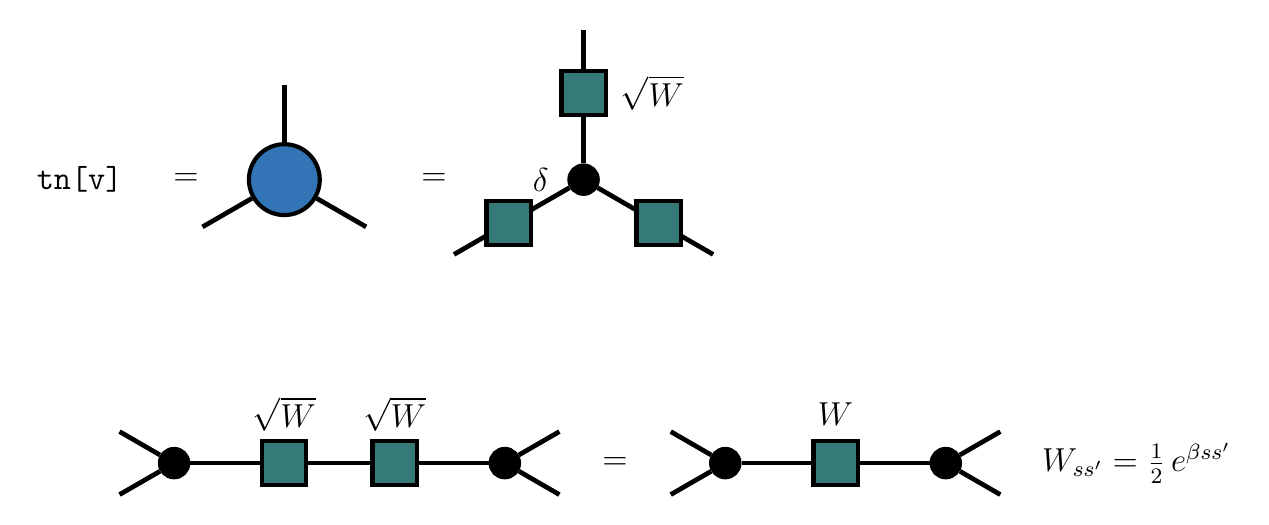
\begin{tikzpicture}
  % Row 1: the tensor on a vertex of degree three
  \node[code] at (-1.2,0) {tn[v]} ;
  \node[lab] at (0.15,0) {$=$};
  \node[tensor] (T) at (1.4,0) {};
  \foreach \a in {90,210,330} { \draw[leg] (T) -- ++(\a:1.2); }
  \node[lab] at (3.3,0) {$=$};
  \node[copy] (d) at (5.2,0) {};
  \foreach \a in {90,210,330} {
    \draw[leg] (d) -- ++(\a:1.9);
    \node[op] at ($(d)+(\a:1.1)$) {};
  }
  \node[lab,anchor=west] at ($(d)+(90:1.1)+(0.35,0)$) {$\sqrt{W}$};
  \node[lab,anchor=east] at ($(d)+(-0.32,0)$) {$\delta$};
  % Row 2: what an edge carries
  \begin{scope}[yshift=-3.6cm]
    \node[copy] (a) at (0,0) {};
    \node[copy] (b) at (4.2,0) {};
    \draw[leg] (a) -- (b);
    \node[op] at (1.4,0) {};
    \node[op] at (2.8,0) {};
    \node[lab] at (1.4,0.62) {$\sqrt{W}$};
    \node[lab] at (2.8,0.62) {$\sqrt{W}$};
    \draw[leg] (a) -- ++(150:0.8); \draw[leg] (a) -- ++(210:0.8);
    \draw[leg] (b) -- ++(30:0.8);  \draw[leg] (b) -- ++(-30:0.8);
    \node[lab] at (5.6,0) {$=$};
    \node[copy] (c) at (7.0,0) {};
    \node[copy] (e) at (9.8,0) {};
    \draw[leg] (c) -- (e);
    \node[op] at (8.4,0) {};
    \node[lab] at (8.4,0.62) {$W$};
    \draw[leg] (c) -- ++(150:0.8); \draw[leg] (c) -- ++(210:0.8);
    \draw[leg] (e) -- ++(30:0.8);  \draw[leg] (e) -- ++(-30:0.8);
    \node[lab,anchor=west] at (10.9,0) {$W_{ss'} = \tfrac{1}{2}\,e^{\beta s s'}$};
  \end{scope}
\end{tikzpicture}
\end{document}
